\section{Gradient Estimation}
\label{section:gradient}
% \hntodo{Provide more context on the main results to expect in this section}

% \hntodo{I think we should explicitly highlight early on, in previous sections (maybe intro) that our smoothing approach is able to compute accurate gradient estimators even in long horizons, and list the extensive nature of our upcoming empirical validation (number policies, envs etc etc).}
In this section, we introduce our proposed approach for estimating the gradient of the objective \eqref{eq:param-cost}, $\nabla J_{N}(\theta)$. We start with a brief discussion of existing methods for gradient estimation, including their advantages and limitations. We then outline the main challenges for computing pathwise derivatives in multi-class queuing networks, and introduce our strategy for overcoming these challenges. Finally, we formally define our gradient estimation framework and discuss its computational and statistical properties. Later in section~\ref{section:gradient_eval}, we perform a comprehensive empirical study and find that our gradient estimation framework is able to overcome many of the limitations of existing methods in that (1) it is capable of estimating gradients for general queuing networks, (2) it provides stable gradient estimations over very long horizons ($>10^5$ steps), (3) it provides greater estimation accuracy than model-free policy gradient methods with 1000x less data, %across 10,800 parameter instances, 
and (4) when applying to policy optimization, it drastically improves the performance of the policy gradient algorithm for various scheduling and admission control tasks. 

\begin{wrapfigure}{L}{0.3\textwidth}
  \begin{center}
  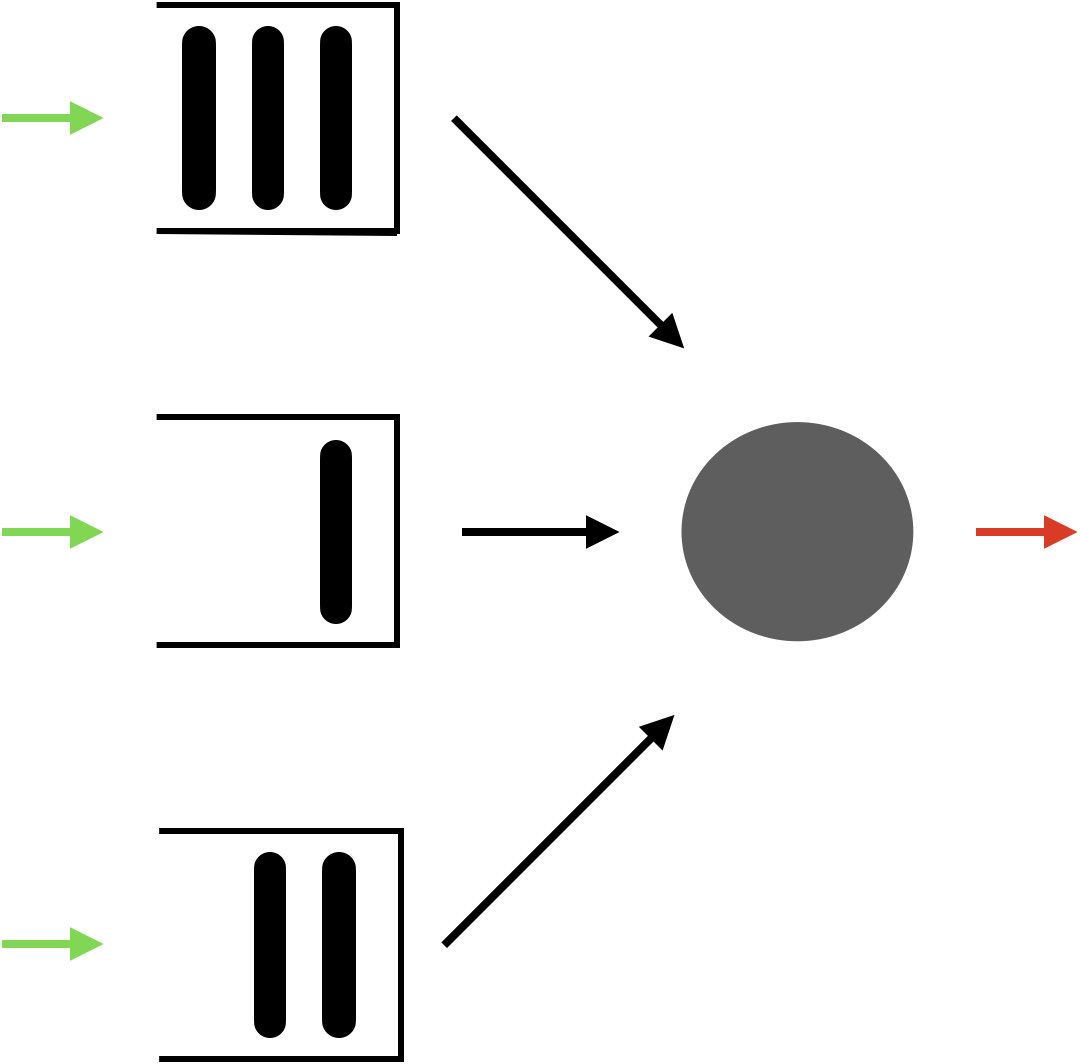
\includegraphics[width=0.2\textwidth]{plot/multiclass.png}
  \end{center}
  \caption{Multi-class, single-server queue.} \label{fig:multi-class}
\end{wrapfigure}

Our goal is to optimize the parameterized control problem (\ref{eq:param-cost}). A standard optimization algorithm is (stochastic) gradient descent, which has been considered for policy optimization and reinforcement learning~\cite{sutton1999policy, baird1998gradient}. The core challenge for estimating policy gradient $\nabla J_{N}(\theta) = \nabla\E\left[J(\theta;\xi_{1:N})\right]$ from sample paths of the queuing network is that the sample path cost $J(\theta, \xi_{1:N})$ is in general not differentiable in $\theta$. As a consequence, one cannot change the order of differentiation and expectation, i.e.,
\[
\nabla J_{N}(\theta)=\nabla\E\left[J_{N}(\theta;\xi_{1:N})\right]\ne\mathbb{E}\left[\nabla J_{N}(\theta;\xi_{1:N})\right],
\]
where $\nabla J_{N}(\theta;\xi_{1:N})$ is not even well-defined.
The non-differentiability of these discrete-event dynamical systems emerges from two sources. First, actions $u_{1:N}$ are discrete scheduling decisions, and small perturbations in the policy can result in large changes in the scheduling decisions produced by the policy. Second, the actions affect the dynamics through the event times. The ordering of events is based on the `$\mathsf{argmin}$' of the residual event times, which is not differentiable.
%This makes it difficult to estimate $\nabla J_{N}(\theta)$ from sample paths.

% \hntodo{We need a 1-2 line math introduction to IPA and LR here. There is no context on what these methods actually do.}
In the stochastic simulation literature, there are two popular methods for gradient estimation: {\bf infinitesimal perturbation analysis} (IPA) and generalized {\bf likelihood ratio} (LR) gradient estimation.
To illustrate, consider abstractly and with a little abuse of notation a system following the dynamics $s_{k+1} = f(s_{k}, \theta, \xi_{k+1})$, where $s_k \in \R$ is the state, $\theta \in \R$ is the parameter of interest,  $\xi_{k}$ is exogenous stochastic noise, and $f$ is a differentiable function. Then, the IPA estimator computes a sample-path derivative estimator
by constructing a derivative process $D_{k}=\partial s_{k} / \partial\theta$ via the recursion:
\[
    D_{k+1} = \frac{\partial}{\partial \theta} f(s_{k}, \theta, \xi_{k+1}) + \frac{\partial}{\partial s_{k}} f(s_{k}, \theta, \xi_{k+1}) \cdot D_{k}
    \tag{IPA}
\]
Likelihood-ratio gradient estimation on the other hand uses knowledge of the distribution of $\xi_{k}$ to form the gradient estimator. Suppose that $s_{k}$ is a Markov chain for which the transition kernel is parameterized by $\theta$, i.e., $s_{k+1} \sim p_{\theta}(\cdot |s_{k})$. %Let $p_{\theta}(s_{k},...,s_{0})=\prod_{j=1}^{k-1} p_{\theta}(s_{j+1}|s_{j})$. 
For a fixed $\theta_{0}$, let 
\[
\frac{\partial}{\partial \theta}\E_{\theta}[s_{k}] = \frac{\partial}{\partial \theta}\E_{\theta_{0}}[s_{k}L_{k}(\theta)] = \E_{\theta_{0}}\left[s_{k}\frac{\partial}{\partial \theta}L_{k}(\theta)\right]
~~\mbox{where}~~L_{k}(\theta) := \frac{\prod_{j=1}^{k-1} p_{\theta}(s_{j+1}|s_{j})}{\prod_{j=1}^{k-1} p_{\theta_0}(s_{j+1}|s_{j})}.
\]
This allows one to obtain the following gradient estimator:
\[
D_{k} = s_{k} \sum_{j=1}^{k-1} 
\frac{\frac{\partial}{\partial \theta}p_{\theta}(s_{j+1}|s_{j})}
{p_{\theta_{0}}(s_{j+1}|s_{j})}L_{k}(\theta), \mbox{ where } s_{j+1} \sim p_{\theta_{0}}(\cdot|s_{j}),\forall j \leq k.
\tag{LR}
\]

Despite their popularity, there are limitations to applying these methods to general multi-class queuing networks. While IPA has been proven efficient for simple queuing models, such as the $G/G/1$ queue through the Lindley recursion, it is well-known that unbiased IPA estimates cannot be obtained for general queuing networks~\cite{cao1987first,fu1994smoothed,fu2012conditional}. The implementation of LR gradient estimation hinges on precise knowledge of the system's Markovian transition kernel ~\cite{glynn1987likelilood}. This requires knowledge of the inter-arrival time and workload distributions, and even with this knowledge, it is non-trivial to specify the transition kernel of the queue lengths and residual event times in generic systems. Modifications to IPA \cite{fu1994smoothed, fu2012conditional} also require precise knowledge of event time distributions and often involve analyzing specific ordering of events which must be done on a case-by-case basis. As a result, none of these methods can reliably provide gradient estimation for complex queuing networks under general scheduling policies and with possibly unknown inter-arrival and service time distributions. Yet, the ability to handle such instances is important to solve large-scale problems arising in many applications.
% While these methodologies have shown to be successful in specific small-scale queueing networks, to the best of our knowledge, neither method can reliably provide gradient estimation for general queueing networks, i.e., under general routing policies with general and possibly unknown inter-arrival and service time distributions. Yet, the ability to handle such instances is important to solve large-scale problems arising in many applications.

Due to the challenges discussed above, existing reinforcement learning (RL) approaches for queueing network control mainly rely on model-free gradient estimators, utilizing either the $\reinforce$ estimator and/or $Q$-function estimation. As we will discuss shortly, these methods do not leverage the structural properties of queuing networks and may be highly sample-inefficient, e.g., requiring a prohibitively large sample for gradient estimation.

To address the challenges discussed above, we propose a novel gradient estimation framework that can handle general, large-scale multi-class queuing networks under any differentiable scheduling policy, requiring only samples of the event times rather than knowledge of their distributions. Most importantly, our approach streamlines the process of gradient estimation, leveraging auto-differentiation libraries such as PyTorch~\citep{PaszkeGrChChYaDeLiDeAnLe17} or Jax~\citep{jax2018github} to automatically compute gradients, rather than constructing these gradients in a bespoke manner for each network as is required for IPA or LR. As shown in Figure~\ref{fig:code}, computing a gradient in our framework requires only a few lines of code. To the best of our knowledge, this is the first scalable alternative to model-free methods for gradient estimation in queuing networks.

% At the same time, by leveraging the known dynamics of queuing networks, we can greatly improve sample efficiency over model-free policy gradient methods, foregoing the need for various hyperparameters and implementation details, such as return normalization, which can often be crucial for the performance and introduce complexity~\cite{engstrom2020implementation}. 

% Despite the discrete nature of the dynamics, this framework leverages knowledge of the queueing network dynamics and provides a simple way to compute derivatives directly through the dynamics, using auto-differentiation libraries such as . To the best of our knowledge, this is the first scalable alternative to $\reinforce$, and as we will demonstrate in the following sections, it can greatly improve upon $\reinforce$ in terms of sample efficiency.

 

\subsection{The standard approach: the $\reinforce$ estimator}
% \hntodo{Nit: let's use $\what{\cdot}$ instead of $\hat{\cdot}$ throughout the paper}

% \hntodo{Explicitly justify why you use REINFORCE as the main baseline. Use soft language like 
% this is a basic proof of concept, so as to not give the impression that we're claiming we're uniformly better than all RL approaches. We can do a bit of this in the abstract + intro.
% }

Considering the lack of differentiability in most reinforcement learning environments, the standard approach for gradient estimation developed in model-free RL is the score-function or $\reinforce$ estimator~\cite{williams1992simple,sutton1999policy}. This serves as the basis for modern policy gradient algorithms such as Trust-Region Policy Optimization (TRPO)~\cite{schulman2015trust} or Proximal Policy Optimization (PPO)~\cite{schulman2017proximal}. As a result, it offers a useful and popular baseline to compare our proposed method with.

 The core idea behind the $\reinforce$ estimator is to introduce a randomized policy $\pi_{\theta}$ and differentiate through the action probabilities induced by the policy. Under mild regularity conditions on $\pi_{\theta}$ and $c(x_k,u_k)$, the following expression holds for the policy gradient:
\[
\nabla J_{N}(\theta) = \mathbb{E}\left[\sum_{t=0}^{N-1} \left(\sum_{k=t}^{N-1}c(x_{k},u_{k})\tau^{*}_{k+1}  \right) \nabla_{\theta}\log \pi_{\theta}(u_{t}|x_{t})\right],
\]
%The term inside the expectation can be estimated pathwise, 
which leads to the following policy gradient estimator:
\begin{equation}
\label{eq:reinforce}
\widehat{\nabla}^{\mathsf{R}} J_{N}(\theta; \xi_{1:N}) = \sum_{t=0}^{N-1} \left(\sum_{k=t}^{N-1}c(x_{k},u_{k})\tau^{*}_{k+1}  \right) \nabla_{\theta}\log \pi_{\theta}(u_{t}|x_{t}).
\hspace{-3em}
\tag{$\reinforce$}
\end{equation}

While being unbiased, the $\mathsf{REINFORCE}$ estimator is known to have a very high variance~\cite{weaver2013optimal}. The variance arises from two sources. First, the cumulative cost $\sum_{k=t}^{N-1}c(x_{k},u_{k})\tau^{*}_{k+1}$ can be very noisy, as has been observed for queuing networks~\cite{dai2022queueing}. Second, 
%when the probabilities $\pi_{\theta}(u_{t}|x_{t})$'s are small, which naturally occurs 
as the policy converges to the optimal policy, the score function $\nabla_{\theta} \log \pi_{\theta}(u_{t}|x_{t})$ can grow large, magnifying the variance in the cost term.  Practical implementations involve many algorithmic add-ons to reduce variance, e.g., adding a `baseline' term~\cite{weaver2013optimal} which is usually (an estimate of) the value function $V_{\pi_{\theta}}(x_{k})$,
\begin{equation}
\label{eq:reinforce_baseline}
\widehat{\nabla}^{\mathsf{RB}} J_{N}(\theta; \xi_{1:N}) = \sum_{t=0}^{N-1} \left(\sum_{k=t}^{N-1}c(x_{k},u_{k})\tau^{*}_{k+1}  
 - V_{\pi_{\theta}}(x_{k})\right) \nabla_{\theta}\log \pi_{\theta}(u_{t}|x_{t}).
 \hspace{-1em}
 \tag{$\mathsf{BASELINE}$}
\end{equation}
These algorithmic add-ons have led to the increased complexity of existing policy gradient implementations~\cite{huang2022cleanrl} and the outsized importance of various hyperparameters~\cite{huang2022implementation}. It has even been observed that seemingly small implementation ``tricks" can have a large impact on performance, even more so than the choice of the algorithm itself~\cite{engstrom2020implementation}.

% To address this challenge, in most applications, the $\mathsf{REINFORCE}$ estimator is averaged across a large number of trajectories. Various variance reduction techniques have also been introduced. One of the common variance reduction strategies is introducing a baseline term, such as value functions estimated using the same sample path. In addition, modern implementations such as Proximal Policy Optimization (PPO)~\cite{schulman2017proximal} or Trust-Region Policy Optimization (TRPO)~\cite{schulman2015trust} put constraints on how far each iterate can move, in large part due to the unreliability of the gradients.\hntodo{This sentence will be too abstract for some readers. Need to specify what "iterates" mean etc. }
% These modifications introduce additional complexity into the gradient estimation process, with standard code implementations of PPO requiring at least 10,000 lines of code split across multiple files~\cite{huang2022cleanrl}. Moreover, the performance of standard policy gradient algorithms can be highly sensitive to  auxiliary implementation details. For example, the clipping ranges and normalization for the rewards and observations having an even larger impact on performance than the choice of RL algorithm itself~\cite{engstrom2020implementation}.  As a result of all these factors, model-free reinforcement learning is often sample-inefficient, computationally-intensive, and fragile~\cite{engstrom2020implementation, ilyas2018closer, huang2022cleanrl, huang2022implementation}.


\subsection{ Our approach: Differentiable Discrete-Event Simulation}

% \hntodo{I think this should be a different section}

%To mitigate these challenges and reliably optimize the control problem \eqref{eq:param-cost}, we develop an alternative framework for gradient estimation. 
% Unlike typical RL settings, where the dynamics of the environment are treated as a black box, queuing networks have structured and known dynamics as described in section \ref{section:model}.
% While the discrete-event representation of the queuing network is primarily used in order to allow for more general inter-arrival and service times.


We can view the state trajectory as a repeated composition of the transition function $s_{k+1} = f(s_{k},u_{k}, \xi_{k+1})$, which is affected by exogenous noise $\xi_{1:N}$, i.e., stochastic inter-arrival and service times. If the transition function were differentiable with respect to the actions $u_{k}$, then under any fixed trace $\xi_{1:N}$, one could compute a \emph{sample-path} derivative of the cost $J(\theta;\xi_{1:N})$ using auto-differentiation frameworks such as PyTorch~\cite{PaszkeGrChChYaDeLiDeAnLe17} or Jax~\cite{jax2018github}. Auto-differentiation software computes gradients efficiently using the chain rule. To illustrate, given a sample path of states, actions, and noise $(s_{k},u_{k},\xi_{k+1})_{k=0}^{N-1}$, we can calculate the gradient of $s_{3}$ with respect to $u_{1}$ via
\[
\frac{\partial s_{3}}{\partial u_{1}} = \frac{\partial s_{3}}{\partial s_{2}} \frac{\partial s_{2}}{\partial u_{1}} =
\frac{\partial f(s_{2},u_{2}, \xi_{3})}{\partial s_{2}} \frac{\partial f(s_{1},u_{1}, \xi_{2})}{\partial u_{1}}.
\]
This computation is streamlined through a technique known as backpropagation, or reverse-mode auto-differentiation. The algorithm involves two steps. The first step, known as the \emph{forward pass}, evaluates the main function or performance metric (in the example, $s_{i}$'s) and records the partial derivatives of all intermediate states relative to their inputs (e.g. $\partial s_{2} / \partial u_{1}$). 
This step constructs a computational graph, which outlines the dependencies among variables. The second step is a \emph{backward pass}, which traverses the computational graph in reverse. It sequentially multiplies and accumulates partial derivatives using the chain rule, propagating these derivatives backward through the graph until the gradient concerning the initial input (in this example, $u_{1}$) is calculated. Due to this design, gradients of functions involving nested compositions can be computed in a time that is linear in the number of compositions. By systematically applying the chain rule in reverse, auto-differentiation avoids the redundancy and computational overhead typically associated with numeric differentiation methods.

However, as mentioned before, the dynamics do not have a meaningful derivative due to the non-differentiability of actions and the $\mathsf{argmin}$ operation which selects the next event based on the minimum residual event time. Yet if we can utilize suitably differentiable surrogates, it would be possible to compute meaningful approximate sample-path derivatives using auto-differentiation.
% Yet, under the discrete-event dynamical system representation, the non-differentiability is isolated in a single operation: the $\mathsf{argmin}$ which selects the next event based off the minimum residual event time.
% \begin{align}
%     e_{k+1} & =\mathsf{argmin}\cup_{i=1}^{n}\{\tau_{k}^{A_{i}},\tau_{k}^{S_{i}}/u_{i}^{\top}\mu_{i}\}\tag{Event Selection}
% \end{align}

\subsubsection{Capacity sharing relaxation} 
% \hntodo{You may get a lot of questions on this relaxation. Discuss in detail whether it's restricting or not restricting. Is it only for learning a policy? Do you present all results in this new formulation so you've effectively changed the name of the game? Does a naive rounding affect performance?}

First, we address the non-differentiability of the action space. Recall that $u_{k} \in \{0,1\}^{m \times n}$ are scheduling decisions, which assign jobs to servers. Since $u_{k}$ lies in a discrete space, a small change in the policy parameters can produce a jump in the actions. To alleviate this, we consider the transportation polytope as a continuous relaxation of the original action space~\eqref{eq:action_space}:
% \begin{equation}
% \label{eq:bar_action_space}
% u_{k} \in \bar{\mathcal{U}} := \left\{u \in [0,1]^{m\times n}: \sum_{i=1}^{m}u_{ij} = 1, \sum_{j=1}^{n}u_{ij} = 1, u \leq M
% \right\}
% \end{equation}
\begin{equation}
\label{eq:bar_action_space}
\overline{\mathcal{U}}:=\left\{ u\in [0,1]^{m\times n}:u\ones_{n} = \ones_{m}, \ones_{m}^{\top} u=\ones_{n},u\leq M\right\}.
\end{equation}
The set of extreme points of $\overline{\mathcal{U}}$ coincide with the original, integral action space $\mathcal{U}$. %However, it is unclear how to interpret 
For a fractional action $u_{k}\in \overline{\mathcal{U}}$, %in the dynamics of the queuing network. We propose a relaxation motivated from fluid models of queuing networks \cite{chen1994hierarchical}: fractional routing decisions represent 
we can interpret it as servers splitting their capacity among multiple job classes motivated by the fluid approximation of queues \cite{chen1994hierarchical}. As a relaxation, it allows servers to serve multiple jobs simultaneously. The effective service rate for each job class is equal to the fraction of the capacity allocated to the job class multiplied by the corresponding service rate. 
%The less capacity allocated to a job, the longer it will take to complete.

As a result, instead of considering stochastic policies over discrete actions, we approach this problem as a \emph{continuous} control problem and consider
\emph{deterministic} policies over continuous actions, i.e., the fractional scheduling decisions. Under this relaxation, the processing times are differentiable in the (fractional) scheduling decision. Finally, it is worth mentioning that we only use this relaxation when training policies. For policy evaluation, we enforce that actions are integral scheduling decisions in $\mathcal{U}$. To do so, we treat the fractional action as a probability distribution and use it to sample a discrete action. 

% \hntodo{Say this earlier, at the beginning of this subsection. Assume that people will view this framework with skepticism, and actively mitigate it by having these sentences up front and center.}
%To reiterate,
\begin{definition}
\label{def:capacity-sharing}
Under the {\bf capacity sharing relaxation}, the service rate for queue $j$ under the routing decision $u\in\overline{\mathcal{U}}$ is $\mu_{j}^\top u_{j} \equiv \sum\nolimits_{i=1}^{m} \mu_{ij}u_{ij}$.
Thus, given workload $w_{j}$, the processing time of the job will be
\begin{equation}
\label{eq:capacity-sharing}
\tau^{S}_{j} =\frac{w_{j}}{\sum_{i=1}^{m}u_{ij}\mu_{ij}} = \frac{w_{j}}{\servicemap_{j,j}}.
\end{equation}
\end{definition}
Note that this is identical to the original definition of the processing times in~\eqref{eqn:processing_time}. The only difference is that we now allow fractional routing actions, under which a server can serve multiple jobs at the same time.


For a concrete example, consider a single server $i$ compatible with two job classes 1 and 2 with service rates $\mu_{i1} = 9$ and $\mu_{i2} = 15$ respectively. Suppose it splits its capacity between job classes 1 and 2 according to $u_{i1} = 1/3$ and $u_{i2} = 2/3$. Then for residual workloads $w_1$ and $w_2$, the corresponding processing times are $\tau^{S}_{1}=w_1/3$ and $\tau^{S}_{2}=w_2/10$. If $u_{i1}=0$ and $u_{i2}=1$ instead, then the corresponding processing times are $\tau^{S}_{1}=w_1/0 = \infty$ and $\tau^{S}_{2}=w_2/15$. %Note that when $u_{k}$ is integral, departure times under the capacity sharing relaxation~\eqref{eq:capacity-sharing} perfectly coincide with departure times under the original, discrete action space.

% Above all, unlike the standard model-free RL approach, which considers stochastic policies $\pi_{\theta}$ that draw actions from the discrete combinatorial action space $\mathcal{U}$, 

% $\pi_{\theta}\in \bar{U}$ that produce fractional routing decisions that determine the effective service rates in a continuous way. 

%{\color{blue} Add an example here.}

\subsubsection{Differentiable event selection}
% \hntodo{Nits: jacobian $\Rightarrow$ Jacobian, iid $\Rightarrow$ i.i.d.}

To determine the next event type, the $\mathsf{argmin}$ operation selects the next event based on the minimum residual event time. This operation does not give a meaningful gradient.

\paragraph{Pitfalls of `naive' smoothing}
In order to compute gradients of the sample path, we need to smooth the $\mathsf{argmin}$ operation. There are multiple ways to do this. A naive approach is to directly replace $\mathsf{argmin}$ with a differentiable surrogate. %Instead of returning a one-hot vector $\{0, 1\}^{2n}$ corresponding to the index of the minimum residual event time, the 
One such popular surrogate is $\softmin$. With some inverse temperature $\beta > 0$, $\softmin_\beta$ applied to the vector of residual event times $\tau \in \R_{+}^{2n}$ returns a vector in $\R_{+}^{2n}$, 
which we use to replace the event selection operation $\event_{k+1}$: 
\begin{equation}
\label{eq:direct_smoothing}
\tilde{\event}_{k+1} = \mathsf{softmin}_{\beta}(\tau_{k})
~~~\mbox{where}~~~\mathsf{softmin_{\beta}(\tau)}_{j}=e^{-\beta \tau_{j}} / \sum_{l=1}^{2n} e^{-\beta \tau_{l}}.
\hspace{-1em}
\tag{Direct Smoothing}
\end{equation}
As $\beta \to \infty$, $\mathsf{softmin}_{\beta}$ converges to $\mathsf{argmin}$. Thus, one may expect that for large $\beta$, $\mathsf{softmin}_{\beta}$ would give a reliable differentiable surrogate. 

However, queuing networks involve a unique challenge for this approach: one typically considers very \emph{long} trajectories when evaluating performance in queuing networks, as one is often interested in long-run average or steady-state behavior. Thus, even if one sets $\beta$ to be very large to closely approximate $\argmin$, the smoothing nonetheless results in `unphysical', real-valued queue lengths instead of integral ones, and small discrepancies can accumulate over these long horizons and lead to entirely different sample paths. 
This can be observed concretely in the left panel of Figure~\ref{fig:naive_smoothing}, which displays the sample paths of the total queueing length processes for a criss-cross queueing network (in Example~\ref{example:criss-cross}) under the original dynamic and under direct smoothing, using the same inter-arrival and service times.  We observe that when setting the inverse temperature $\beta = 1$, the sample path under direct smoothing is completely different from the original one, even though all of the stochastic inputs are the same. 
%The sample path is much smoother. 
Even when setting a very high inverse temperature, i.e., $\beta = 1000$, for which $\mathsf{softmin}_{\beta}$ is almost identical to $\mathsf{argmin}$, the trajectory veers off after only a hundred steps. 

\begin{figure}[t]
\centering
    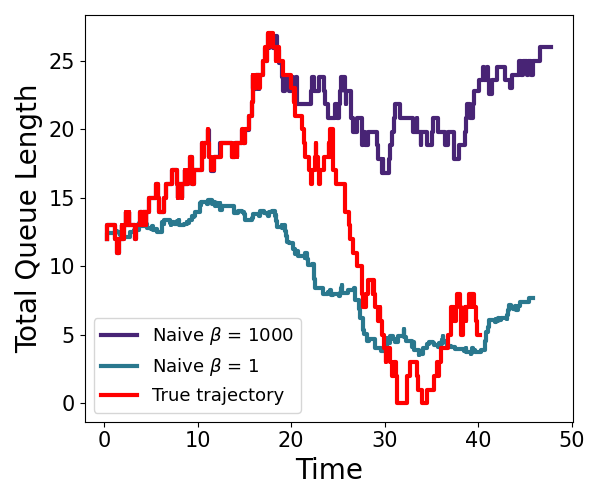
\includegraphics[height = 2.2in]{plot/gradient/compare_naive_smoothing.png}
    % \hspace{0.1em}
    % 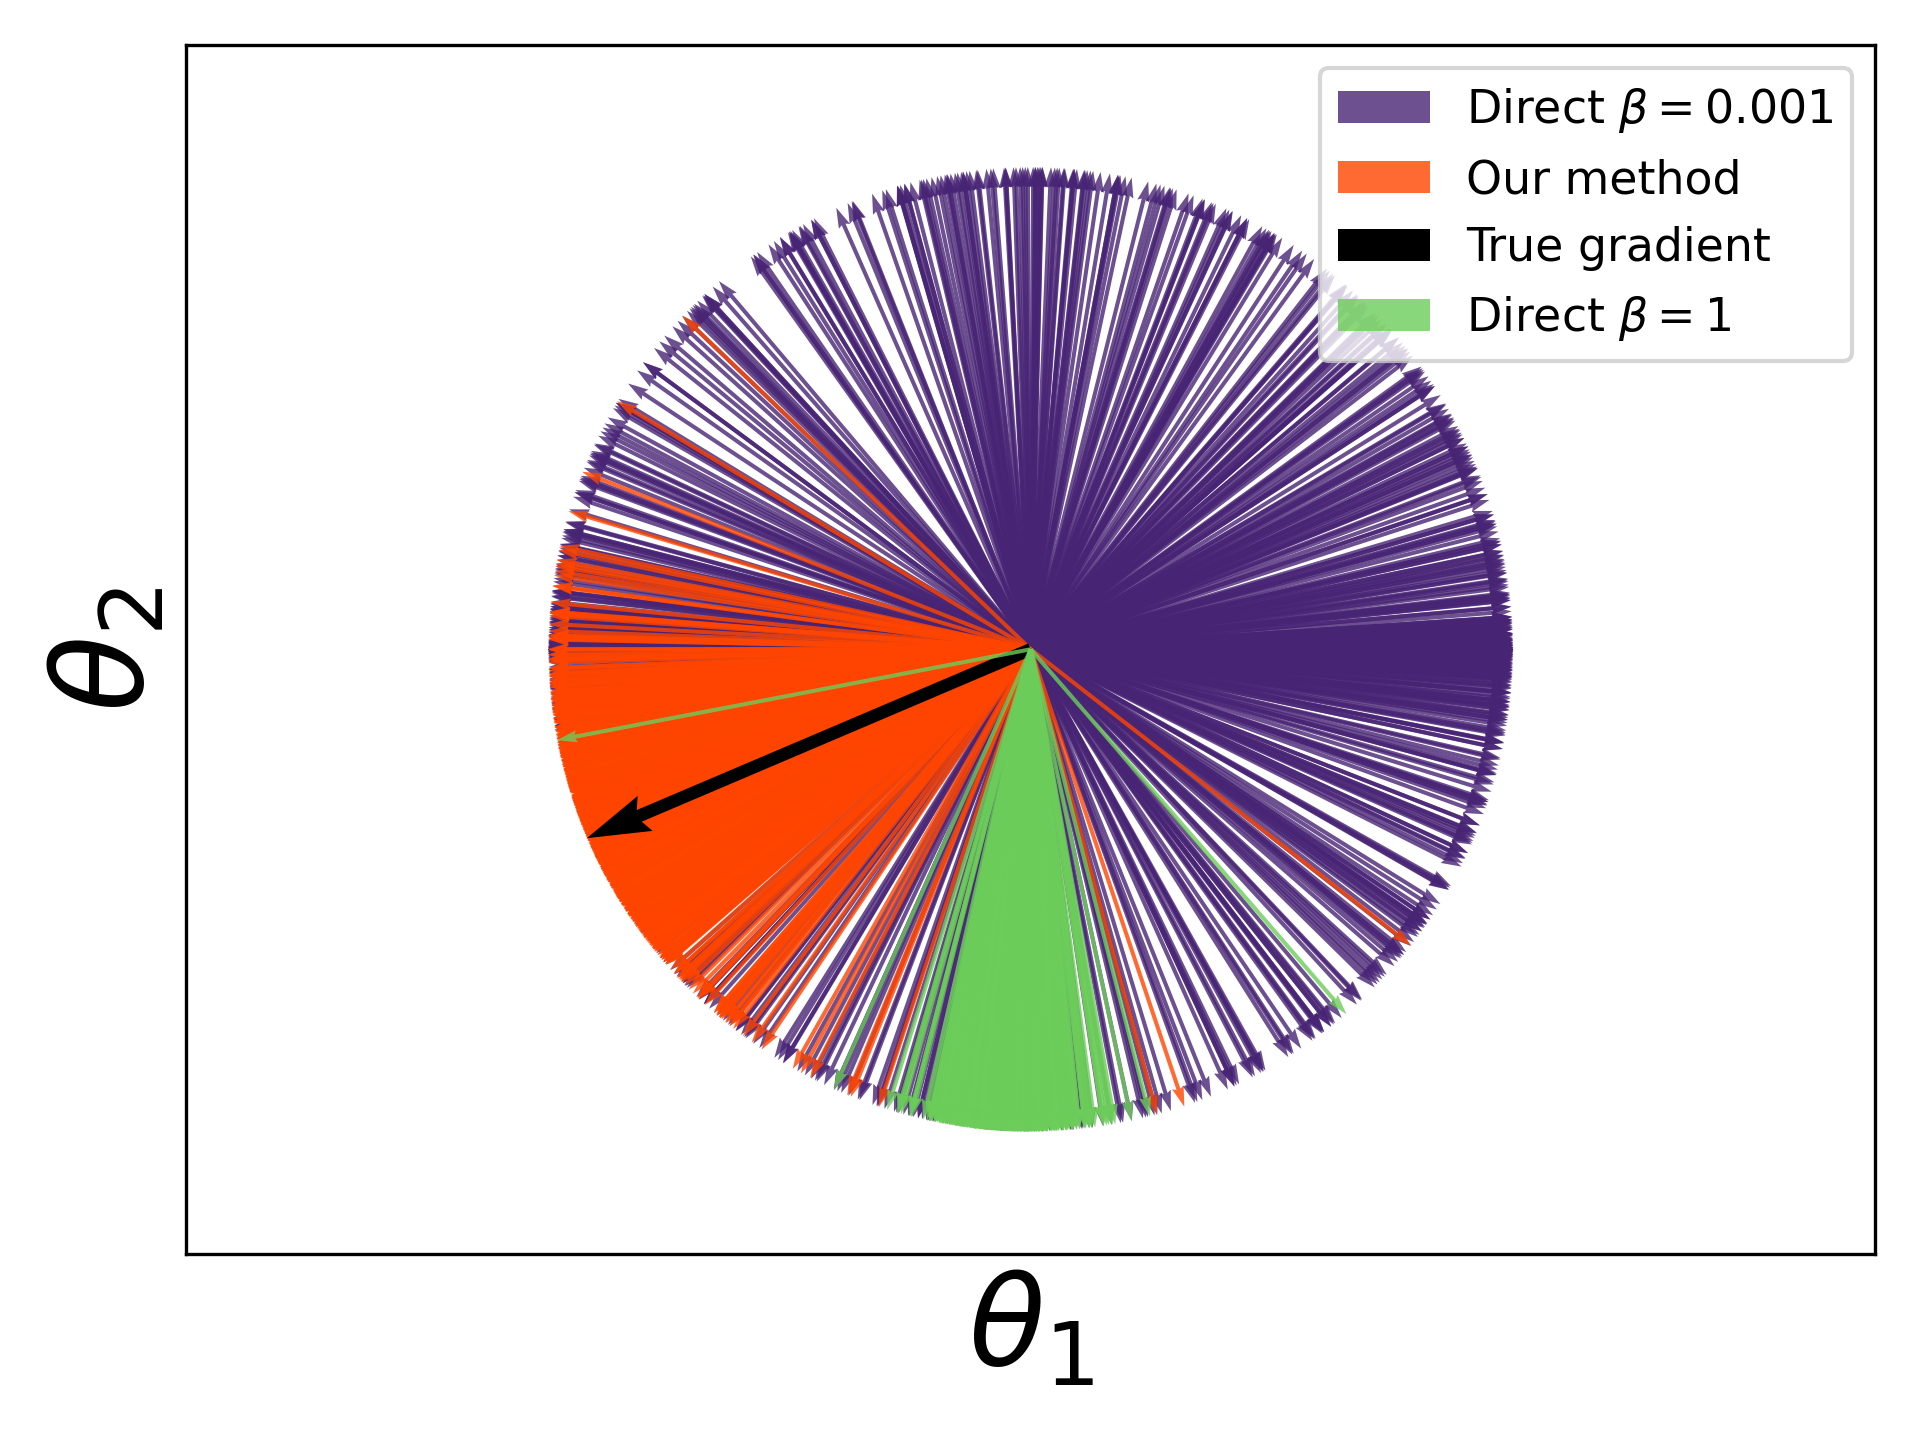
\includegraphics[height = 1.6in]{plot/gradient/direct_smoothing_vectors.png}
    \hspace{0.1em}
    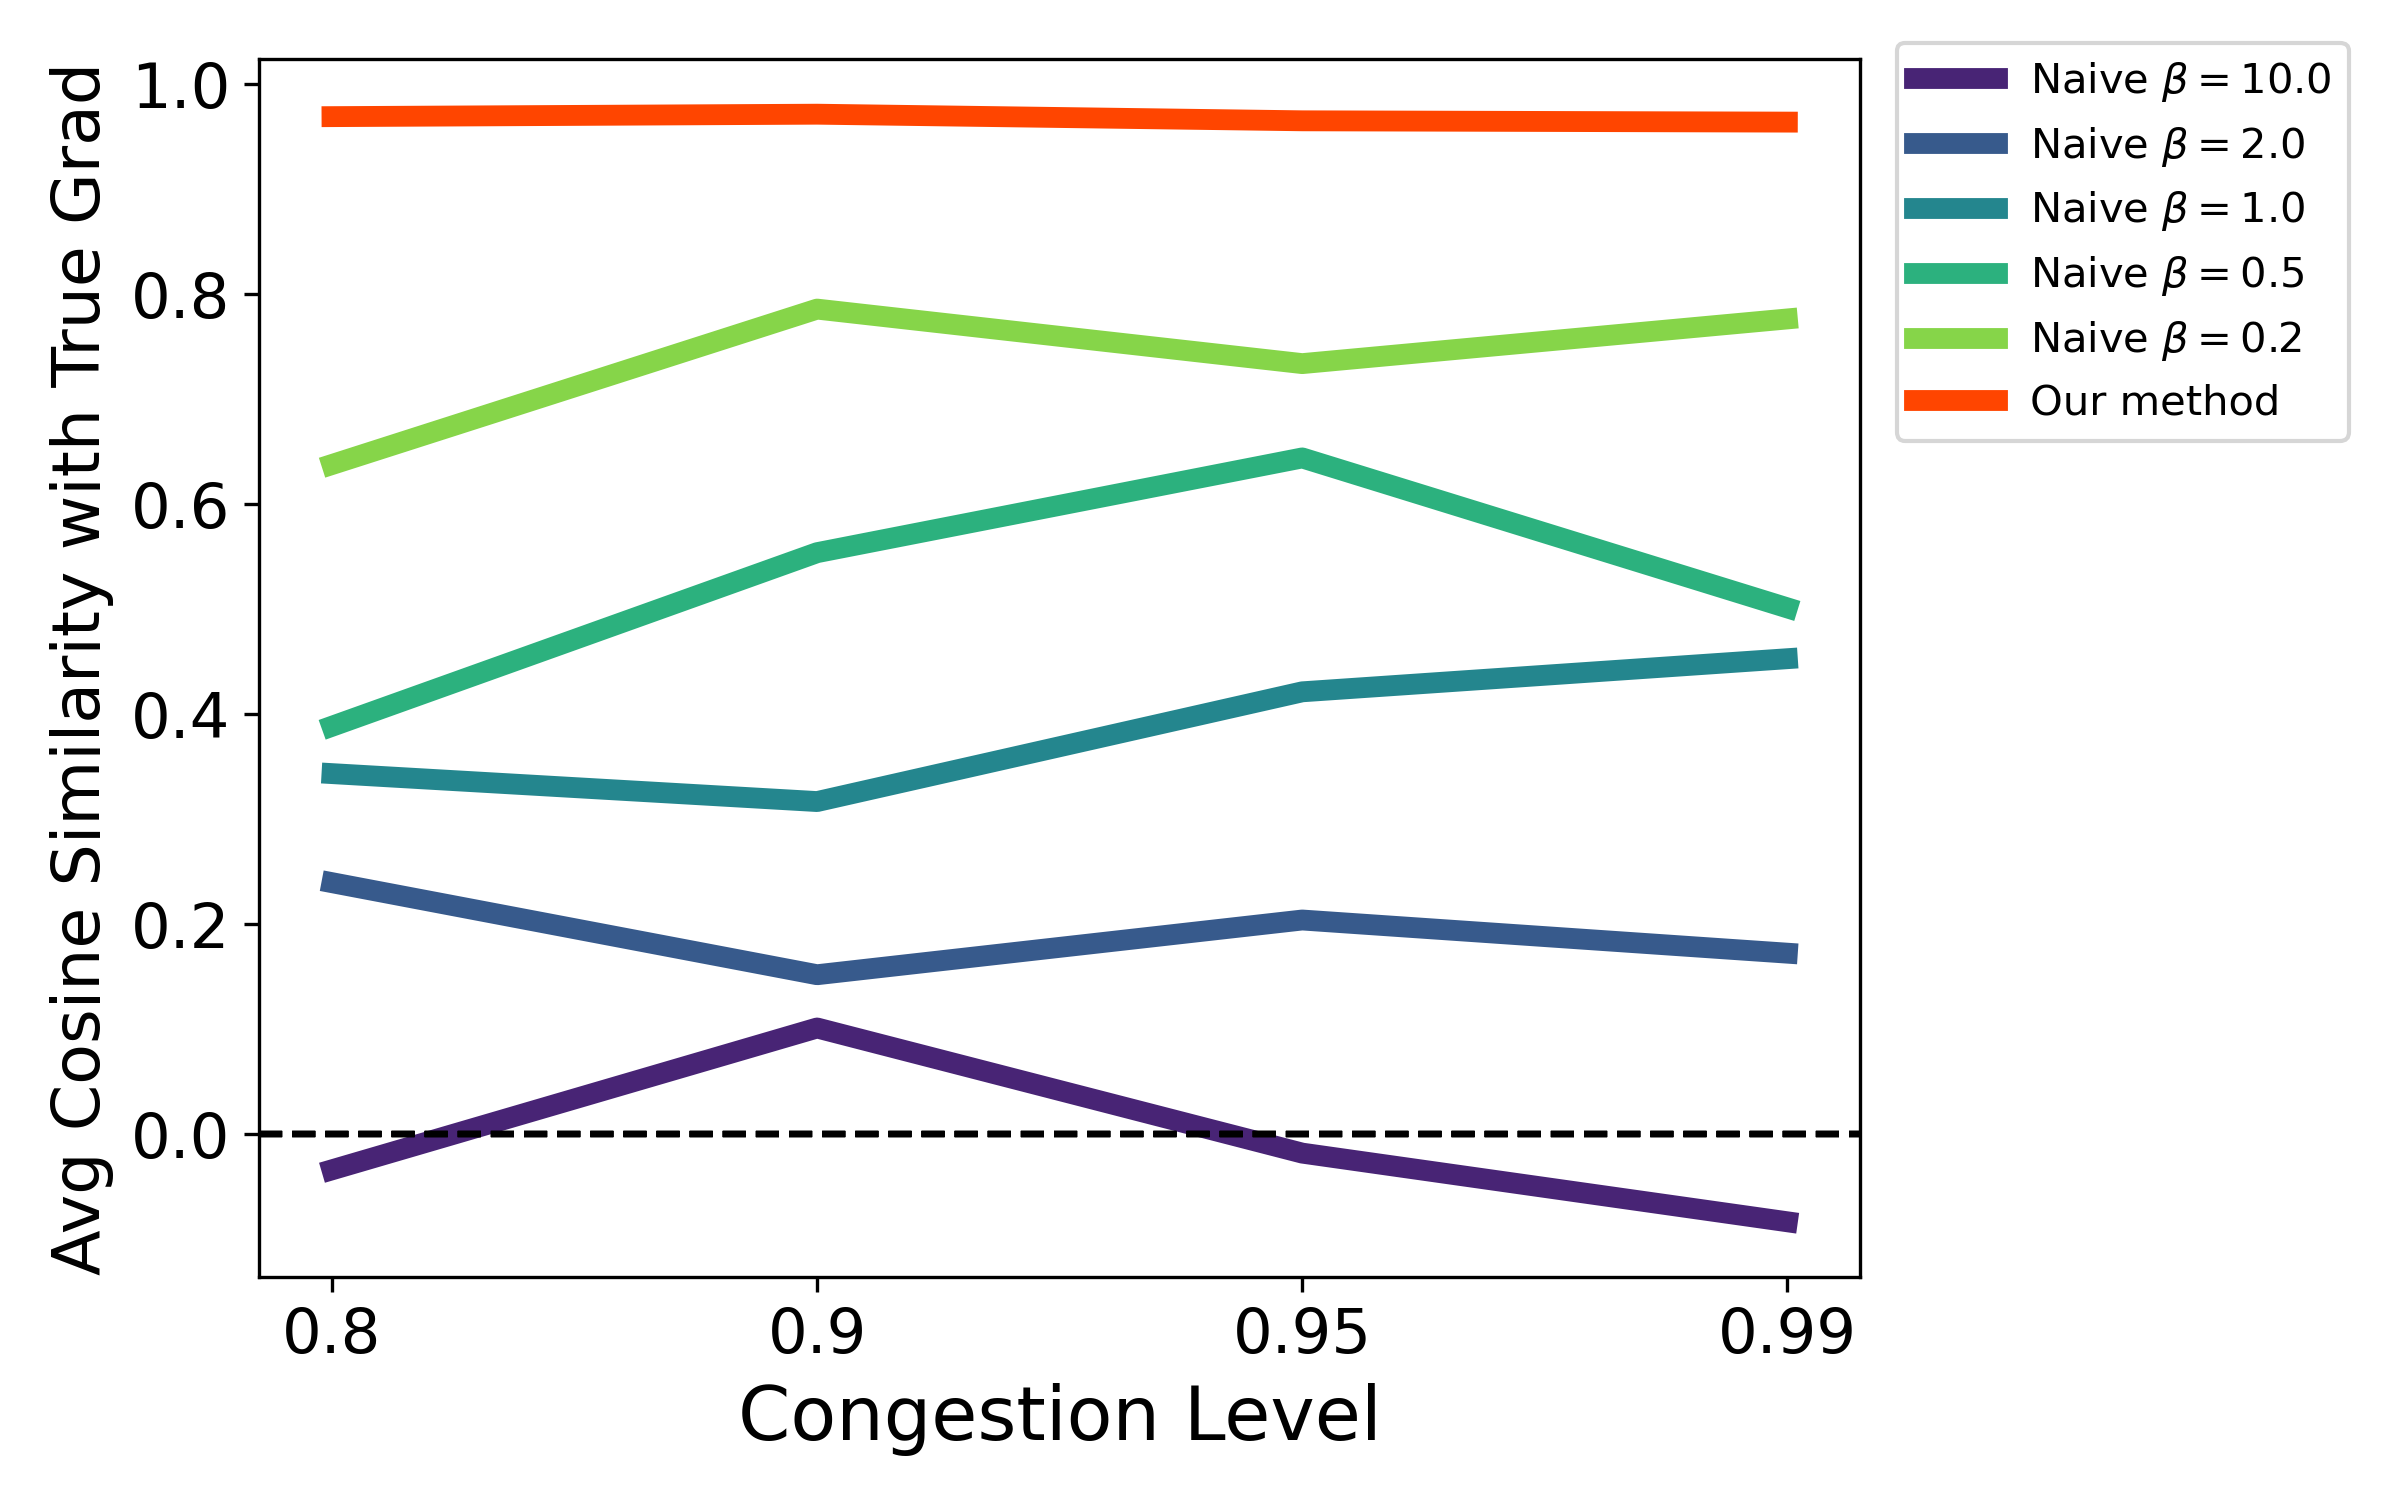
\includegraphics[height = 2.2in]{plot/gradient/naive_smoothing_cos.png}
    
    \caption{Failure modes of `naive' smoothing. (Left) Comparison of sample paths under the original dynamics and direct smoothing with $\beta = 1$ and $\beta = 1000$. Criss-cross network under a randomized backpressure policy with identical event times in each path, for $N = 200$ steps. 
    Even under high inverse temperature $\beta = 1000$, the trajectory veers off from the original trajectory after only a hundred steps. 
    % (Middle) Samples of policy gradient estimators for the randomized backpressure policy in the criss-cross network estimated along a horizon of $N = 1000$. The true gradient (in black) is estimated by averaging the $\mathsf{REINFORCE}$ estimator over $10^{7}$ trajectories. 
    % Direct smoothing for $\beta = 1$ has low variance but is biased. Direct smoothing with $\beta = 1000$ has a prohibitively high variance. Our proposed method greatly reduces bias while maintaining a low variance.
    (Right) Comparison of average cosine similarity (higher is better) of gradient estimators using direct smoothing with $\beta  \in \{0.2, 0.5, 1, 2, 10\}$ for the criss-cross network under a randomized MaxWeight policy for $N = 1000$ steps. 
    The gradient estimators either suffer from high bias or high variance and are unable to achieve a high cosine similarity with the true gradient.
    }
    \label{fig:naive_smoothing}
\end{figure}


This can greatly affect the quality of the gradient estimation. 
%The middle panel of Figure~\ref{fig:naive_smoothing} displays samples of the smoothed gradient estimator for a policy gradient task. Direct smoothing under $\beta = 1$ leads to a low-variance but biased estimator. Yet, if we set $\beta = 10$, the variance can be large and the gradient estimator does not reliably point in any direction. This points to a trade-off that prevents reliable gradient estimation: low inverse temperatures bias the gradient estimates whereas high inverse temperatures lead to numerical instabilities. Even if this hyper-parameter is carefully tuned, the estimators either have too high a bias or variance rather than reaching a meaningful tradeoff. For example,
We observe in the right panel of Figure~\ref{fig:naive_smoothing} that across a range of inverse temperatures, the average cosine similarity between the surrogate gradient and the true gradient (defined in \eqref{eqn:similarity}) are all somewhat low.
%the estimators either have too high a bias or variance rather than reaching a meaningful tradeoff. 
In the same plot, we also show the average cosine similarity between our proposed gradient estimator, which we will discuss shortly, and the true gradient. Our proposed approach substantially improves the gradient estimation accuracy, i.e., the average cosine similarity is close to $1$, and as we will show later, it does so across a wide range of inverse temperatures. %Overall this illustrates the unique challenges that emerge for constructing differentiable simulators of discrete dynamical environments. 
% In the machine learning literature, smoothing techniques for gradient estimation have typically been applied to tasks such as density estimation or structured prediction~\cite{maddison2016concrete,jang2017categorical}, which are one-period problems that do not involve repeated smoothing across a trajectory. 
% Recently, \cite{petersen2021learning} develop differentiable relaxations for algorithms (such as sorting or shortest path) by applying differentiable relaxations for discrete operations. 
% Most relevant for our work, \cite{andelfinger2021differentiable, andelfinger2023towards} propose differentiable agent-based simulators based on differentiable relaxations, but find that while they helped achieve strong performance on optimization tasks, these relaxations also created unpredictable discrepancies with the original dynamics. Reliable simulation involved carefully balancing the trade-off in the level of smoothing in order to balance fidelity to the original environment with reliability of the gradient estimates. These considerations are especially crucial for queuing networks, as reliably estimating steady-state quantities requires rolling out the dynamics for horizons ranging from $N = 10,000$ to even $N= 100,000$ steps.

\paragraph{Our approach: `straight-through' estimation}

The failure of the direct smoothing approach highlights the importance of preserving the original dynamics, as errors can quickly build up even if the differentiable surrogate is only slightly off. We propose a simple but crucial adjustment to the direct smoothing approach, which leads to huge improvements in the quality of gradient estimation. 
% \hntodo{Notice how you don't mention how you pick $\beta$ until the very end of this section. Again, assume by default that people will be skeptical of your highly novel and innovative empirical framework. Actively take measures to mitigate concerns. I would put the paragraph on insensitive against $\beta$ and the corresponding empirical plots front and center, right after you introduce "our method"}

Instead of replacing the $\mathsf{argmin}$ operation with $\mathsf{softmin}_{\beta}$ when generating the sample path, we preserve the original dynamics as is, and only replace the Jacobian of $\mathsf{argmin}$ with the Jacobian of $\softmin_\beta$ when we query gradients. In short, we introduce a gradient operator $\widehat{\nabla}$ such that
\begin{equation}
\event_{k+1}=\mathsf{argmin}(\tau_{k}), \quad \quad
\widehat{\nabla} \event_{k+1}= \nabla \softmin_{\beta}(\tau_{k}). 
\end{equation}
where $\nabla$ is respect to the input $\tau$.
%while $\widehat{\nabla}$ is equivalent to standard gradient operator for all other differentiable functions.
% Plot of maybe MM1 (or something more complicated). Our method gets the right gradient, but direct smoothing gets something crazy.
%  Our approach is to preserve the $\mathsf{argmin}(\tau)$ in the forward pass of dynamics, when we roll out the dynamics on a particular sample path, but replace with the $\mathsf{softmin_{\beta}(\tau)}=e^{\beta \tau_{j}} / \sum_{j=1}^{2n} e^{\beta \tau_{j}}$ operation when computing
% To overcome this issue, we apply a differentiable surrogate in a careful manner. We maintain the $\mathsf{argmin}$ operation when generating the sample path to preserve the original dynamics exactly as is. It is only when we query gradients, that we then replace the jacobian of $\mathsf{argmin}$ with the jacobian of the $\softmin$ operation, defined as
% $\mathsf{softmin_{\beta}(\tau)}=e^{-\beta \tau_{j}} / \sum_{i=1}^{2n} e^{-\beta \tau_{i}}$, so that:
% \begin{equation}
% \event_{k+1}=\argmin(\nu(\tau_{k}, u_{k})), \quad \quad
% \nabla \event_{k+1}= \nabla \softmin_{\beta}(\nu(\tau_{k}, u_{k})) 
% \end{equation}
This is known as the `straight-through' trick in the machine learning literature and is a standard approach for computing approximate gradients in discrete environments~\cite{bengio2013estimating, van2017neural}. To the best of our knowledge, this is the first application of this gradient estimation strategy for discrete-event dynamical systems. Using this strategy, we can use the chain rule to compute gradients of performance metrics that depend on the event selection. 
% We denote $\widehat{\nabla}$ to be the corresponding gradient operator. 
Consider any differentiable function $g$ of $e_{k+1}$, 
%(e.g. a holding cost for the queue lengths which is updated by the event selection):
\[
\widehat{\nabla} g(\event_{k+1}) = \frac{\partial g(\event_{k+1})}{\partial \event_{k+1}} \widehat{\nabla} \event_{k+1} \nabla \tau_{k}= \frac{\partial g(\event_{k+1})}{\partial \event_{k+1}} \nabla \softmin_{\beta}(\tau_{k}) \nabla \tau_{k}
\]
In contrast, direct smoothing involves the derivative $\partial g(\tilde{e}_{k+1})/\partial \tilde{e}_{k+1}$ where $\tilde{e}_{k+1} = \softmin_{\beta}(\tau_{k})$.  Evaluating the gradient of $g$ at $g(\tilde{e}_{k+1})$ is a cause of additional bias.
% \hntodo{I also often see that because OR/MS does not have a well-developed empirical rigor standard (e.g., in contrast to top-tier LLM research these days), there is a default belief that anything empirical must be viewed with skepticism and that most researchers are not thorough (in some cases that they are sometimes even dishonest). We'd do well to explicitly highlight many times throughout the paper (starting in the introduction and abstract) how systematic and comprehensive your evaluations are. Think of concrete numbers and figures you can say, e.g., number of environments, number of policy params etc etc.}

%\subsubsection{Come up with a title for this}
With these relaxations, the transition function of the system is differentiable. We can now compute a gradient of the sample path cost $J_{N}(\theta; \xi_{1:N})$, using the chain rule on the transition functions. Given a sample path of states $s_{k} = (x_{k}, \aux_{k})$, actions $u_{k} = \pi_{\theta}(x_{k})$, and $\xi_{k} = (T_{k}, W_{k})$, the pathwise gradient of the sample path cost is $J_{N}(\theta; \xi_{1:N})$ with respect to an action $u_{k}$ is,
\[
\widehat{\nabla}_{u_{k}} J_{N}(\theta; \xi_{1:N})
= \underbrace{\nabla_{u_{k}}c(x_{k},u_{k})}_{\text{current cost}} + \sum_{t=k+1}^{N} 
\left[  \underbrace{ \nabla_{x}c(x_{t}, u_t) + \nabla_{u} c(x_{t}, u_t)\nabla_{x_{t}}\pi_{\theta}(x_{t})}_{\text{future costs}} \right]
\nabla_{u_{k}}x_{t}
\]
The gradient consists of the sensitivity of the current cost with respect to the action as well the sensitivity of future costs via the current action's impact on future states. The policy gradient with respect to $\theta$ can then be computed as
\begin{equation}
\label{eq:pathwise-pg}
\widehat{\nabla}_{\theta} J_{N}(\theta; \xi_{1:N}) = \sum_{k=1}^{N} \left. \widehat{\nabla}_{u_{k}} J_{N}(\theta; \xi_{1:N}) \right|_{u_{k} = \pi_{\theta}(x_{k})} \nabla_{\theta} \pi_{\theta}(x_{k}).
\hspace{-3em}
\tag{$\pathwise$}
\end{equation}
As a result of the straight-through trick, we do not alter the event selection operation $\event_{k}$'s and thus the state trajectory $\{x_{k} \}_{k=1}^{N}$ is unchanged.

% \hntodo{We should highlight this point way earlier, starting in Section 1, but also throughout Sections 2-3. We need to accentuate the computational nature of our regimen. Until very recently, taking these gradients required hand-coding them in, but now we have extremely effective ways to do auto-differentiation. This is precisely why the reader had to go through the cumbersome notation in the entirety of Section 2. Once you have the entire problem in matrix-vector notation, we basically have a "pseudo-code" for our method. This point should come out in Sections 1 and 2.} 

We refer to the gradient estimator \eqref{eq:pathwise-pg} as the $\mathsf{PATHWISE}$ {\bf policy gradient estimator}. Although this formula involves iterated products of several gradient expressions, these can be computed efficiently through reverse-mode auto-differentiation using libraries such as PyTorch~\cite{PaszkeGrChChYaDeLiDeAnLe17} or Jax~\cite{jax2018github} with $O(N)$ time complexity in the time horizon $N$. This time complexity is of the same order as the forward pass, i.e., generating the sample path itself, and is equivalent to the time complexity of $\mathsf{REINFORCE}$. The policy gradient algorithm with $\mathsf{PATHWISE}$ gradient is summarized in Algorithm \ref{alg:pathwise-pg}. In Section~\ref{section:gradient_eval}, we perform a careful empirical comparison of $\pathwise$ and $\reinforce$, and find that $\pathwise$ can lead to orders of magnitude improvements in sample efficiency. 
% Although the straight-through method preserves the sample path on which we evaluate the gradient, it is still unclear whether this will result in an effective gradient estimator, since we are still using a surrogate gradient.
%inputting a surrogate gradient in-place of the uninformative gradient of the $\argmin$ at every step. 
% Later in section~\ref{section:gradient_eval}, we empirically investigate the statistical properties of the gradients, namely whether
% \[
% \E[\widehat{\nabla}_{\theta} J_{N}(\theta; \xi_{1:N})]
% \approx \nabla_{\theta} J_{N}(\theta) \quad \text{and} \quad 
% \var(\widehat{\nabla}_{\theta} J_{N}(\theta; \xi_{1:N})) < \var(\widehat{\nabla}^{\mathsf{R}}_{\theta} J_{N}(\theta; \xi_{1:N}))
% \]
% \hntodo{I don't think this is the right algo box to state. I recommend coming up with a visual scheme of iteratively applying $f$'s and illustrating the straight-through in the same figure. }

\begin{algorithm}[t]
  \caption{\label{alg:pathwise-pg} $\pathwise$ Policy Gradient ($\mathsf{PathPG}$) }
  \begin{algorithmic}[1]
    \State \textsc{Input: Policy $\pi_{\theta}$, Number of Iterates $T$, horizon $N$, trace $\xi_{1:N}$, step-size $\alpha>0$}.
    \For{each $t \in 1, \ldots, T$}
    \State Compute $J_{N}(\theta;\xi_{1:N}) = \sum_{k=1}^{N} c(x_{k}, \pi_{\theta}(x_{k})) \tau_{k+1}^{*}$ from trace $\xi_{1:N}$.
    \State Compute gradient $\widehat{\nabla}_{\theta} J_{N}(\theta; \xi_{1:N})$ via~\eqref{eq:pathwise-pg}
    \State Update policy parameters,
    \[
    \theta_{t+1} \leftarrow \theta_{t} - \alpha \widehat{\nabla}_{\theta} J_{N}(\theta; \xi_{1:N})
    \]
    \EndFor 
    \State \Return $\pi_{\theta_{T}}$
  \end{algorithmic}
\end{algorithm}

% \hntodo{Again, from the skepticism view, I would err on the side of stating this early on. I also found this paragraph quite confusing because it is unclear what the difference between evaluating a policy vs. model is.}
It is important to re-emphasize that when computing the gradient, we evaluate the policy differently than we would for $\reinforce$. Instead of drawing a random discrete action $u_{k} \sim \pi_{\theta}(x)$, we use the probabilities output by the policy directly as a fractional routing matrix in $\overline{\mathcal{U}}$,
\begin{align*}
\reinforce:& \quad u_{k} \sim \pi_{\theta}(x_{k}),\qquad u_{k} \in \mathcal{U} \\
\pathwise:& \quad u_{k} = \pi_{\theta}(x_{k}),\qquad u_{k} \in \overline{\mathcal{U}}.
\end{align*}
However, this is only for gradient computation. When we evaluate the policy, we draw $u_{k} \sim \pi_{\theta}(x_{k})$.

\begin{figure}[t]
    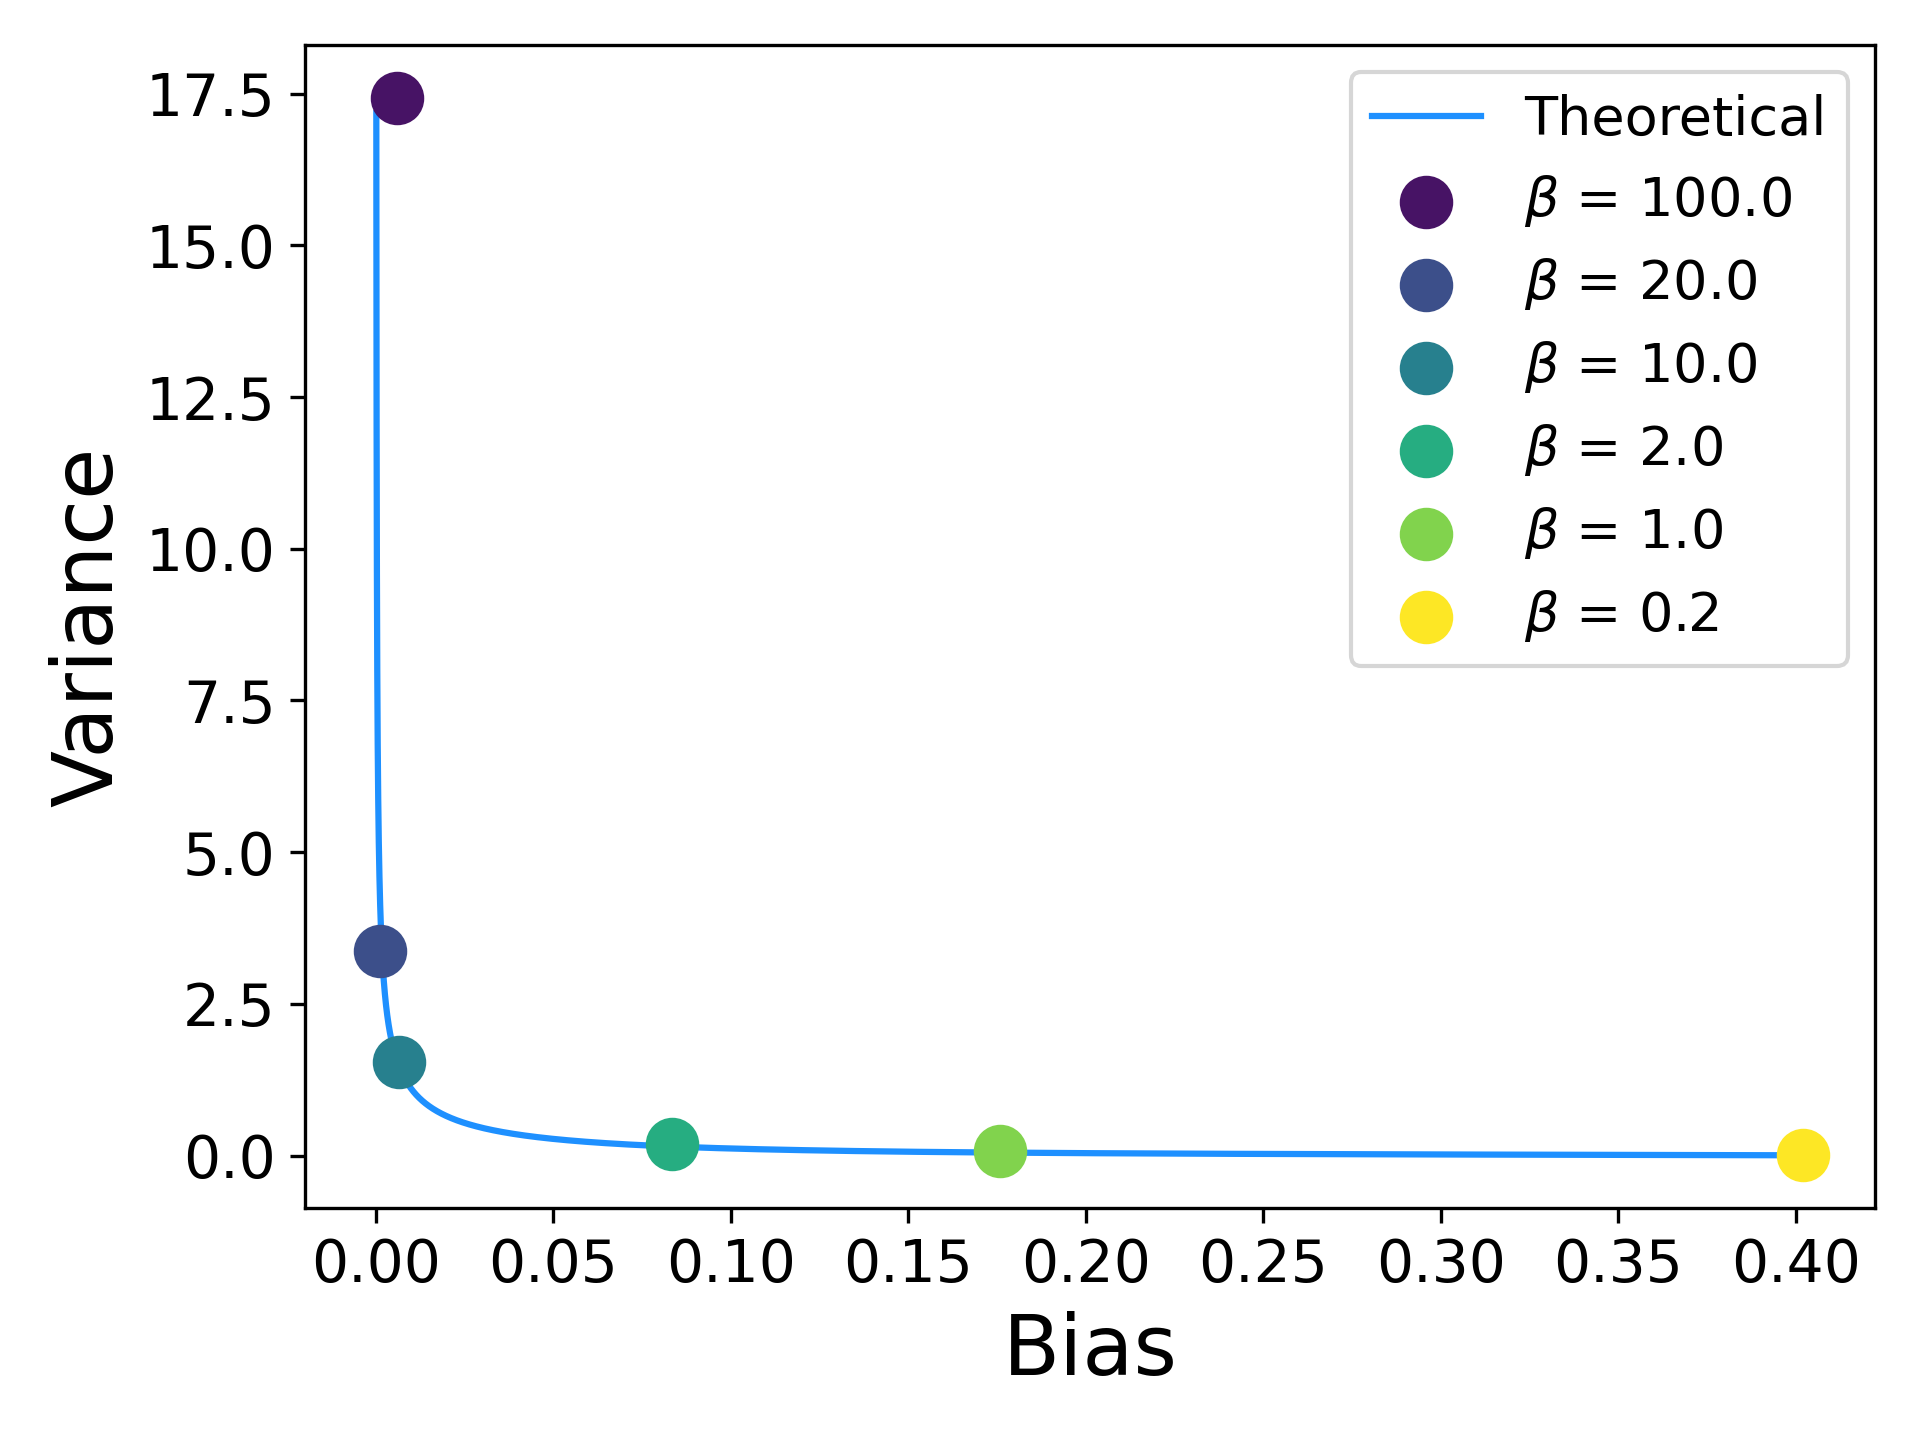
\includegraphics[height = 2.3in]{plot/gradient/bias_variance_one_step.png}
    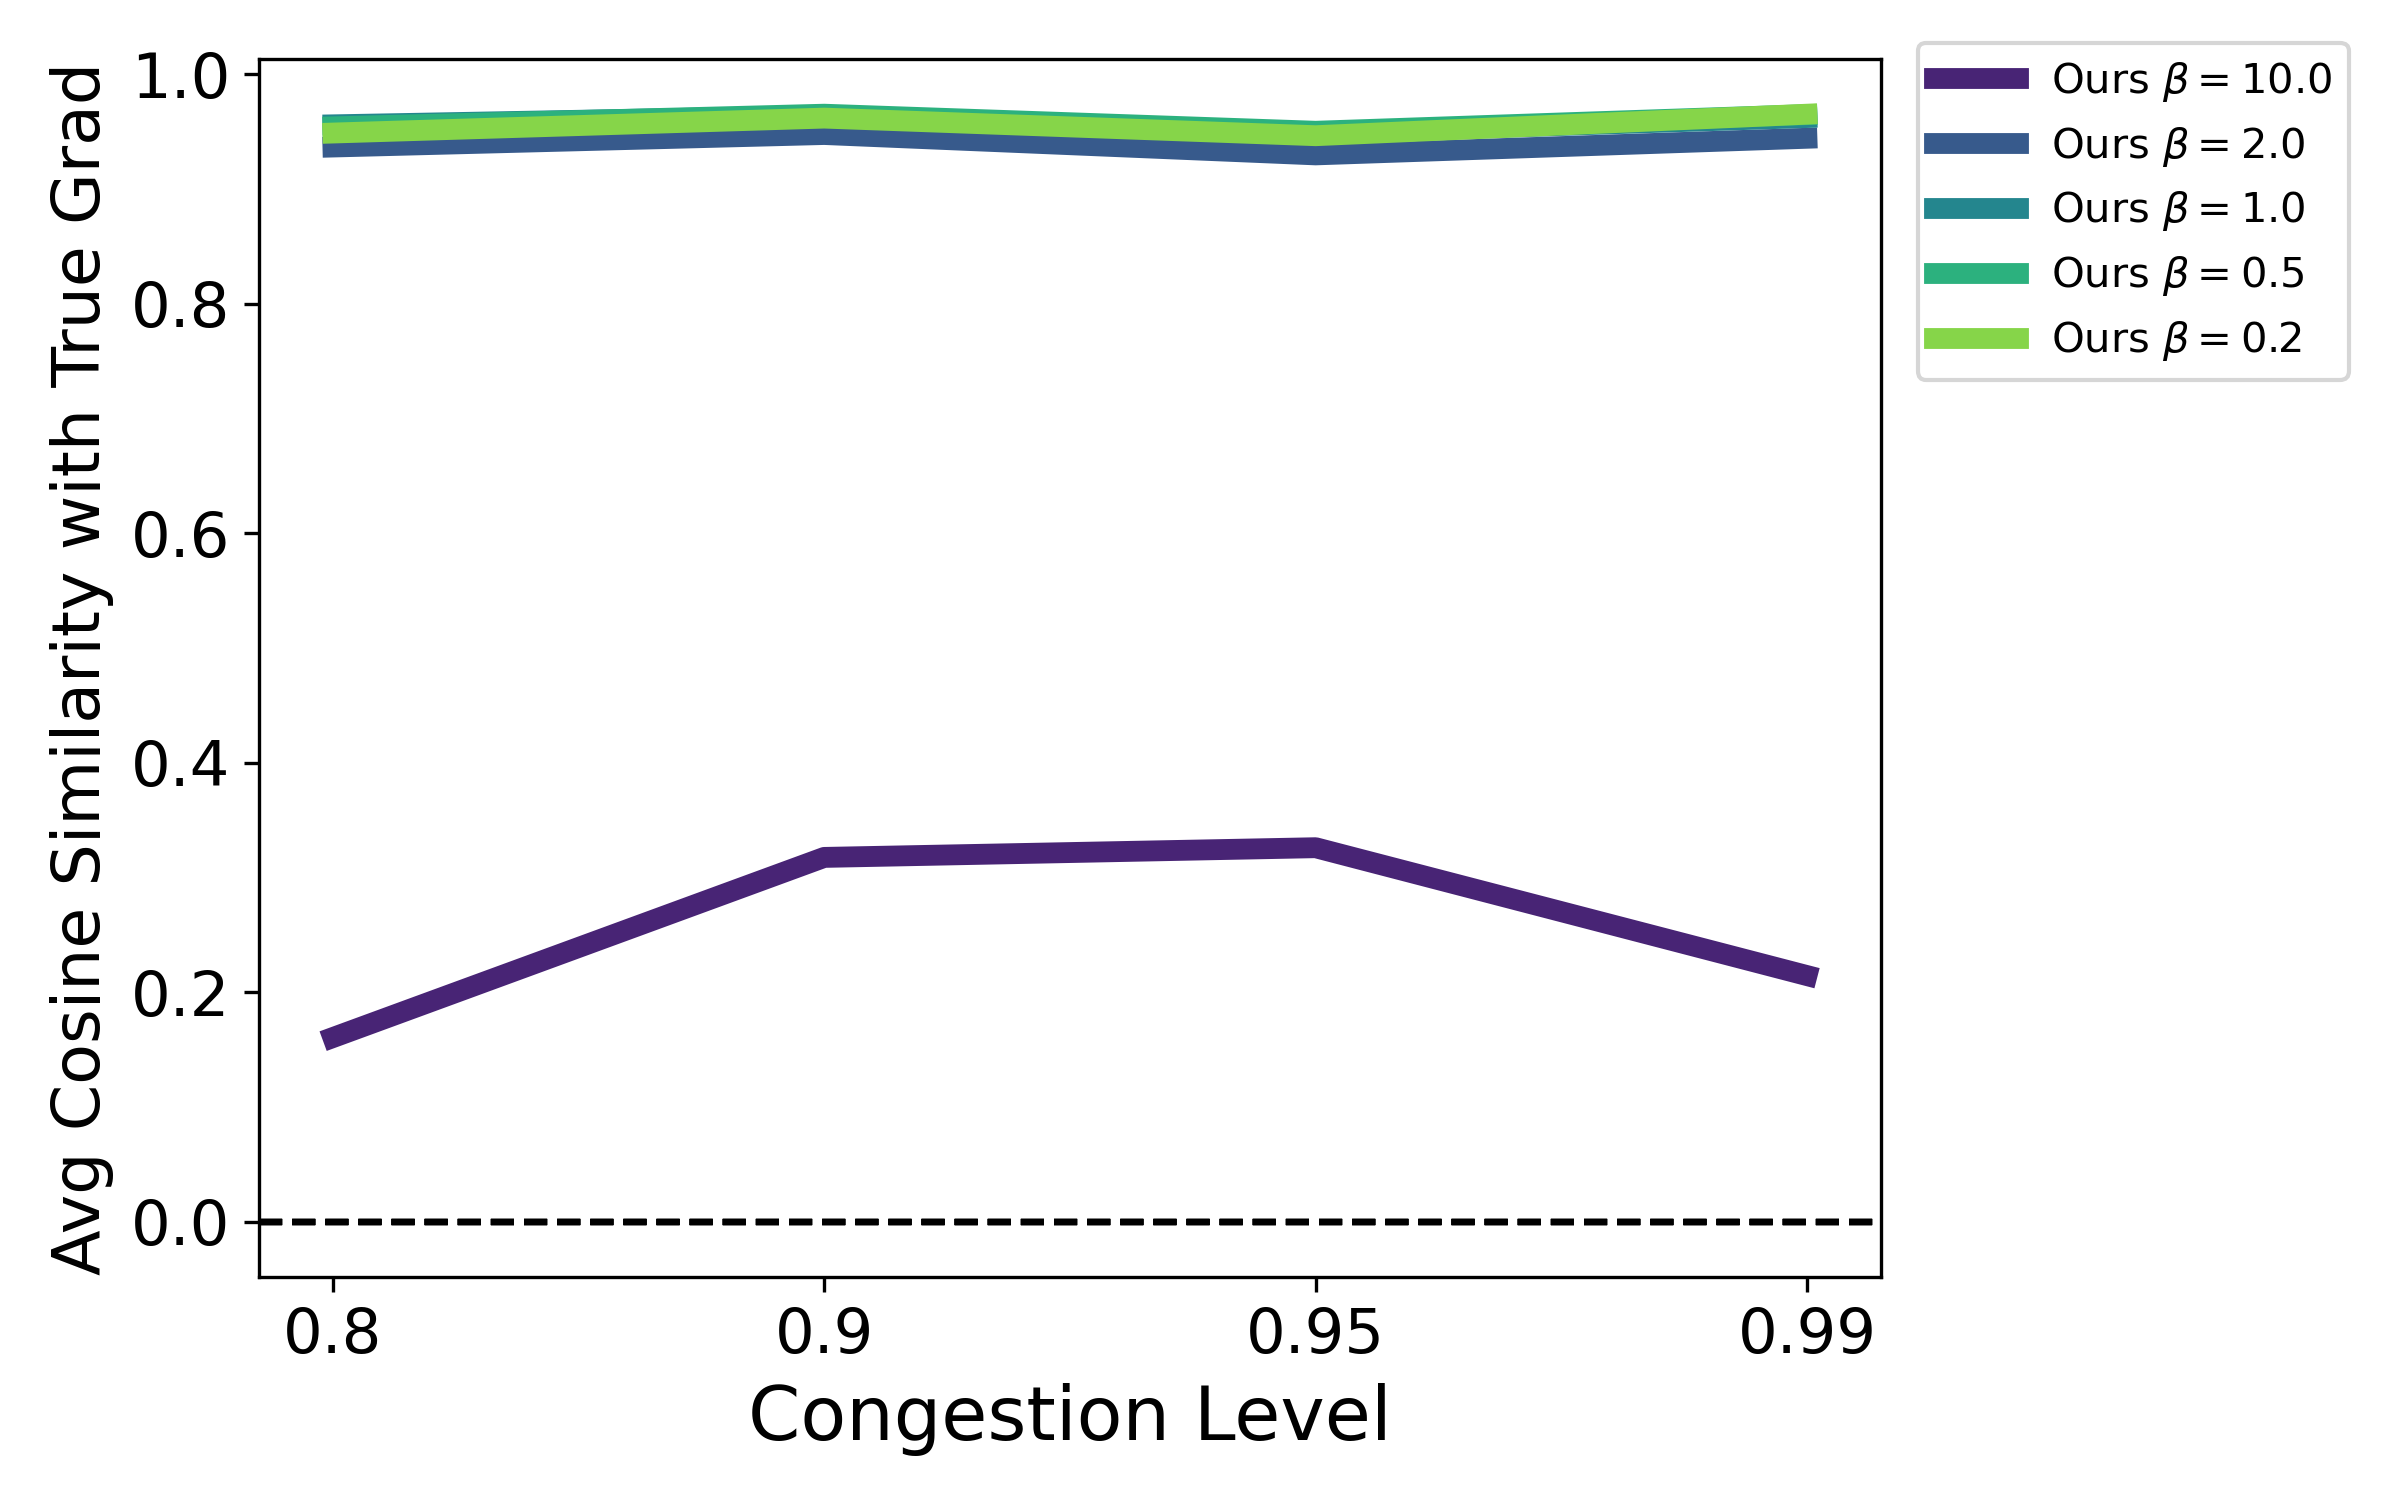
\includegraphics[height = 2.3in]{plot/gradient/our_smoothing_cos.png}
    
    \caption{Bias-variance trade-off for inverse temperature $\beta$. (Left) Bias and variance of pathwise gradient estimator across a range of inverse temperatures $\beta$ for the one-step change $\widehat{\nabla}_{\mu}(x_{k+1} - x_{k})$ compared to true gradient $\nabla_{\mu}\E[x_{k+1} - x_{k}] = \nabla_{\mu}\frac{\lambda - \mu}{\lambda + \mu}$. Blue line specifies the theoretical values for the bias and variance. (Right) Average cosine similarity (see~\eqref{eqn:similarity} for the definition) of $\pathwise$ policy gradients with the true gradient for a randomized max-weight policy (see~\eqref{eqn:soft_policies}) in a 6-class reentrant network (see Figure~\ref{fig:networks}) across a range of inverse temperatures computed from a single trajectory $B = 1$ for $N = 1000$ steps. True gradient is computed by averaging $\reinforce$ over $10^{6}$ trajectories. $\pathwise$ gradient has almost a perfect cosine similarity $\approx 1$ across a wide range of inverse temperatures.}
    \label{fig:bias-variance} 
\end{figure}

\paragraph{Bias-variance trade-off for inverse temperature: One-step analysis}
The inverse temperature $\beta$ is a key hyperparameter that determines the fidelity of the $\softmin_{\beta}$ approximation to $\argmin$. The choice of $\beta$ poses a bias-variance trade-off, with a higher $\beta$ leading to a smaller bias but a higher variance and a smaller $\beta$ incurring a higher bias but a lower variance. 

In general, it is difficult to assess the bias since we  often do not know the true gradient. However, for some simple examples, we can evaluate the true gradient explicitly. We next analyze the gradient of the one-step transition of the $M/M/1$ queue with respect to the service rate $\mu$,
\[
\nabla_{\mu}\E[x_{k+1} - x_{k}]=  \nabla_{\mu} \E[D e_{k+1}] =\nabla_{\mu}\frac{\lambda - \mu}{\lambda + \mu} = -2\frac{\lambda}{(\lambda + \mu)^{2}}.
\]
This permits an exact calculation of the mean and variance of our proposed pathwise gradient estimator. Although we can derive analytical expressions for these quantities, we present the leading order asymptotics as $\beta \to \infty$ for conciseness of presentation. While it is straightforward to see that almost surely $\softmin_{\beta}(\tau)\to \argmin(\tau)$ as $\beta \to \infty$, it is much less clear whether the gradient converges, i.e., whether $\E[\nabla \softmin_{\beta}(\tau)] \to \nabla \E[\argmin(\tau)]$. Since $\argmin$ has a gradient of zero almost everywhere, the expectation and gradient operators cannot be interchanged. 
%Using a pointwise convergence argument would lead to an incorrect gradient of zero. 
Instead, we analyze the expectations directly using properties of the exponential distribution.
\begin{theorem}
\label{thm:mm1-smoothing}
Let $\widehat{\nabla}_\mu (x_{k+1} - x_{k}) =  \widehat{\nabla}_\mu De_{k+1}$ denote the $\mathsf{PATHWISE}$ gradient estimator of the one-step transition of the $M/M/1$ queue with respect to $\mu$.  For $x_k\geq 1$, as $\beta \to \infty$,
\begin{align*}
\E[\widehat{\nabla}_\mu De_{k+1}]
-\nabla_\mu \E[ De_{k+1}]
&= \beta^{-2} \cdot \frac{\pi^{2}\lambda (\mu^{2} - \lambda^{2} + 2\mu \lambda)}{6(\lambda + \mu)^{2}}
+ o \left( \beta^{-2} \right), \\
\var(\widehat{\nabla}_\mu De_{k+1})
&= \beta \cdot \frac{4\lambda}{\mu (\lambda + \mu)^{2}} + o(\beta).
\end{align*}
\end{theorem}
See section~\ref{section:mm1-smoothing-proof} for the proof.
As $\beta \to \infty$, the bias is $O(1/\beta^{2})$ while the variance is $O(\beta)$. This means that one can significantly reduce the bias with only a moderate size of $\beta$. The left panel of Figure~\ref{fig:bias-variance} shows the bias-variance trade-off of $\widehat{\nabla}_\mu (x_{k+1} - x_{k})$ for various inverse temperatures $\beta$. The blue line is based on the analytical expression for the bias-variance trade-off curve. We observe that with the inverse temperature $\beta \in [0.5, 2]$, both the bias and the variance are reasonably small.
%the bias can be made to be small with only a mild increase in variance



%The favorable bias-variance trade-off translates into sample efficiency of the gradient estimator, as can be seen in Corollary~\ref{cor:one-step-mse}.
\begin{corollary}
\label{cor:one-step-mse}
Suppose we compute the sample average of $B$ iid samples of $\widehat{\nabla}_{\mu} De_{k+1}$, which are denoted as $\widehat{\nabla}_{\mu} De_{k+1, i}$, $i=1,\dots, K$. In particular, the estimator takes the form $\frac{1}{B}\sum_{i=1}^{B} \widehat{\nabla}_{\mu} De_{k+1,i}$. The choice of $\beta$ that minimizes the mean-squared error (MSE) of the estimator 
%$\text{MSE}(\beta) := \text{Bias}(\beta)^{2} + \text{Variance}(\beta)/B$ 
is $\beta^{*} = O(B^{1/5})$ and $\text{MSE}(\beta^*)=O(B^{-4/5})$.
\end{corollary}



The $\pathwise$ estimator provides a more statistically efficient trade-off than other alternatives. As an example, a standard gradient estimator is the finite-difference estimator in which one evaluates the one-step transition at $\mu - h$ and $\mu + h$ for some small $h \in (0,\infty)$, and the estimator is constructed as
\[
\frac{1}{B}\sum_{i=1}^{B} \frac{De_{k+1,i}(\mu + h) - De_{k+1,i}(\mu - h)}{2h},
\]
where $De_{k+1,i}(\mu + h)$'s are iid samples of $De_{k+1}(\mu + h)$.
If we set $h = 1/\beta$, it is well-known that the bias scales as $O(1/\beta^{2})$ while the variance scales as $O(\beta^{2})$. The choice of $\beta$ that minimizes the MSE is $\beta^{*} = O(B^{1/6})$ and $\text{MSE}(\beta^*)=O(B^{-1/3})$.

% \hntodo{State before theory, say many times in the introduction and subsequent sections that our approach is practically insensitive to smoothing parameter so long as you use straight-through. Reiterate and forward reference to empirical validations to come.}
While this analysis is restricted to the one-step transition of the $M/M/1$ queue, these insights hold for more general systems and control problems. The right panel of Figure~\ref{fig:bias-variance} displays the average cosine similarity (defined in ~\eqref{eqn:similarity}) between the $\pathwise$ gradient estimator and the true gradient for a policy gradient task in a 6-class reentrant network across different congestion levels and for different inverse temperatures. We observe that for a wide range of inverse temperatures, $\beta \in \{0.2, 0.5, 1, 2\}$, the estimator has near-perfect similarity with the true gradient, while a very large inverse temperature suffers due to high variance. This indicates that while there is a bias-variance trade-off, the performance of the $\pathwise$ gradient estimator is not sensitive to the choice of the inverse temperature within a reasonable range. In our numerical experiments, we %fix $\beta = 10$ or $\beta = 1$ and 
find that one can get good performance using the same inverse temperature across different settings without the need to tune it for each setting. 
%{\color{blue} We also conduct a case study comparing the sample efficiency of $\reinforce$ and $\pathwise$ for the $M/M/1$ queue in section \ref{section:case_study}.}

% \hntodo{From the viewpoint of mitigating skepticism, this figure is dangerously misleading. We've been differentiating between Direct vs ours so far, yet it appears that we now use "Direct" to mean ours. We should always denote "Ours $\beta$" vs. "Direct $\beta$" to differentiate between straight-through, even in single step problems where the distinction doesn't matter. It is easy for casual readers to miss these things.

% Moreover, it is genuinely difficult for people to grasp that $\beta = 10$ is already a pretty extreme value, and that $\beta = 100$ is an incredibly large number. Casual readers (unfortunately sometimes even referees) will think that if you plot 6 lines without much explicit context and see half of them suck, then the method is sensitive and problematic.}
% One can contrast this with the standard discrete-time MDP representation, in which the transition function is determined by a draw from a discrete probability distribution: $s_{t+1} \sim P(\cdot | s_{t},u_{t})$.